\chapter{Описание практической части}

\section{Выбранный инструментарий}

Для реализации использовался язык программирования Python версии 3.8, который был выбран в силу своего удобство и простоты. Также важным преимуществом этого языка является наличие множества дополнительных программных модулей с открытым программным кодом.\\
Проект включает в себя Python-скрипты, а также Jupyter блокноты. Jupyter - среда для интерактивного программирование, которое упрощает осуществление экспериментов.\\
В качестве ключевых фреймворков и программных модулей, используемых для реализации проекта, можно выделить:
\begin{itemize}
\item PyTorch \cite{NEURIPS2019_9015} - популярный фреймворк для создания и обучения нейросетей, разрабатываемые компанией Facebook. Ему было отдано предпочтение, потому что, в отличие от его единственного конкурента TensorFlow, PyTorch обладает качественными документацией и программным интерфейсом, что делает разработку и поддержание моделей более простым и удобным;
\item Scikit-learn \cite{scikit-learn} - программный модуль, содержащий в себе огромное количество различных классических алгоритмов машинного обучения и различные средства обработки данных. Был взят именно он, потому что является де-факто стандартом в своей сфере;
\item Pandas \cite{mckinney-proc-scipy-2010} - модуль для работы со табличными массивами данных. Используется, так как предлагает множество инструментов, облегчающие работу с csv-файлами из набора данных;
\item Dask \cite{dask} - модуль для параллелизированной обработки данных. Имеет программный интерфейс схожий с Pandas. Предназначен для агрегации данных с контентом, размеры которых превышают доступную оперативную память на рабочей машине;
\item Ignite - надстройка для PyTorch, упрощающая написание процесса обучения и валидации моделей;
\item GenSim \cite{rehurek_lrec} - модуль для работы с текстовыми данными. Взят, так как он способен работать с огромными массивами текстовых данных, которые не способны уместиться в оперативной памяти;
\item TensorBoard - модуль для логирования обучения моделей. Так как является частью проекта TensorFlow, используется модуль TensorBoardX, который предоставляет программный интерфейс для любых фреймворков;
\item Weights and Biases \cite{wandb} - сервис для сбора логов и результатов экспериментов и их последующей визуализации. Для этого предоставляется Python модуль wandb.
\end{itemize}

За неимением адекватной видеокарты, для обучения нейросетей используется сервис Google Colaboratory, который предоставляет бесплатный доступ к онлайн Jupyter-ноутбукам в средах с доступом к производительным GPU. Сервис обладает рядом ограничений на время работы и зачастую сервис нестабилен, но для обучения рассматриваемых моделей этого достаточно.

\section{Сценарии функционирования}

Проект включает в себя один базовый сценарий построения моделей машинного обучения для классификации пользовательского поведения и проведения экспериментальных исследований. Этот сценарий разбивается на несколько:
\begin{itemize}
	\item Составление признакового описания данных;
	\item Обучение SkipGram-модели;
	\item Обучение LSTM-кодировщика;
	\item Обучение CNN-классификатора.
\end{itemize}

% TODO Написать про SkipGram в обзоре

Для обучения любых моделей требуются подготовленные признаковые описания данных. На этом же этапе происходит разделение данные на тренировочные и валидационные подвыборки. Обучение SkipGram моделей используется как опциональный компонент, в то время как для обучения CNN-классификатора, требуется уже обученная LSTM-модель. Обучение всех моделей происходит по эпохам. В конце каждой тренировочной эпохи вычисляются метрики по тренировочной и валидационной подвыборках. Все полученные метрики собираются в лог-файл. Также в конце каждой эпохи происходит сохранение полученных весов моделей, если модель является лучшей по валидационной метрике. Обучение продолжается до тех пор, пока количество эпох не превысит вручную заданный порог, или в случае, если в последние N эпох валидационные метрики не улучшались (техника, которая называется ``ранней остановкой'').

\section{Архитектура разработанного средства}

Разработанный проект делится на подготовленные программные модули, в которых описываются тестируемые модели, конфигурации, схема обработки данных, процесс обучения моделей. Также есть Jupyter-тетради, в которых происходят эксперименты с моделями в интерактивном режиме.\\
На \autoref{fig:architecture} условно отображена архитектура программного средства. В круглых облаках написаны названия классов, направленные стрелки обозначают наследование классов, а не направленные - ассоциацию классов. В пунктирных коробках отображаются Jupyter-тетради, в которых проводятся эксперименты и используемые методы из других модулей.

% TODO: update line count
Всего написано \textbf{2443} строк кода, которые включают в себя \textbf{1034} строк в python-скриптах и суммарно \textbf{1409} строк кода в ячейках Jupyter-тетрадей.\\

\begin{figure}[ht]
	\noindent\makebox[\textwidth]{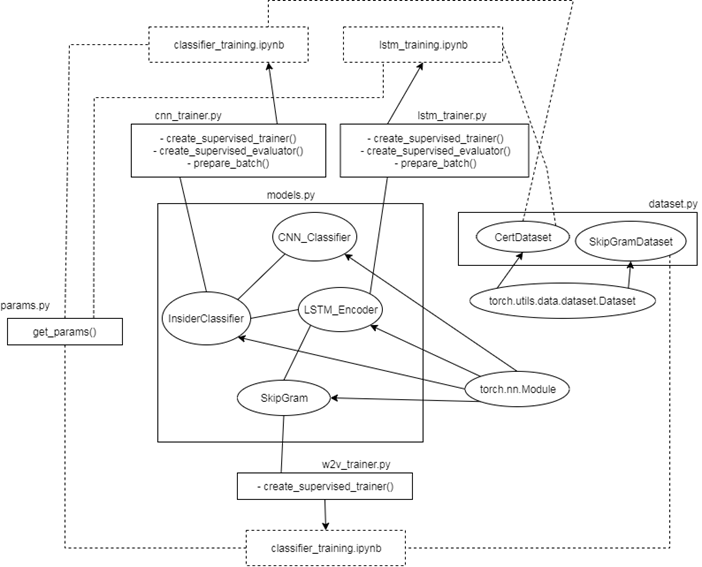
\includegraphics[width=\linewidth]{architecture-scheme}}
	\caption{Архитектура разработанного средства}
	\label{fig:architecture}
\end{figure}

Разработанные программные модули:
\begin{itemize}
\item Для каждого типа обучаемых нейросетей, есть \textit{``xxx\_trainer.py''} скрипт, который описывает процессы обучения и валидации модели. С помощью средств модуля Ignite устанавливаются функции обратного вызова и события, при которых они вызываются. С помощью этих функций происходит вычисление вспомогательных метрик, TensorBoard логирование, сохранение на жёсткий диск промежуточных, финальных и лучших по валидации весов модели. Скрипты обладают функциями \textit{create\_supervised\_trainer()} описывающие процесс тренировки; \textit{create\_supervised\_evaluator()}, которая описывает процесс валидации и \textit{prepare\_batch()}, описывающее процесс обработки полученных данных для текущей задачи. Каждому скрипту соответствует файл Jupyter-тетради \textit{``xxx\_training.ipynb''} в которых проводятся эксперименты с соответствующей моделью.
\item{``\textit{dataset.py}''} описывает обработку данных. Реализовано два класса: \textit{CertDataset} и \textit{SkipGramDataset} для обучения классификатора и SkipGram модели соответственно. Оба класса наследуются от класса \textit{utils.data.dataset.Dataset} из фреймворка Pytorch.
\item ``\textit{models.py}'', который описывает архитектуру обучаемых моделей. Каждая модель задаётся специальным Python-классом, унаследованным от класса из пакета Pytorch nn.Module. В каждом классе описываются методы \textit{\_init\_()} (конструктор, в котором описываются поля объекта и задаются слои модели) и \textit{forward()}, в которой происходит обработка объектов, поступивших на вход модели. Реализованные классы: \textit{CNN\_Classifier}, \textit{LSTM\_Encoder}, \textit{InsiderClassifier} и \textit{SkipGram}, которые описывают CNN-классификатор, LSTM-кодировщик, классификатор инсайдерского поведения целиком и SkipGram-модель соответственно. \textit{InsiderClassifier} содержит в себе модели \textit{CNN\_Classifier} и \textit{LSTM\_Encoder}.
\item ``\textit{params.py}'' - содержит в себе конфигурацию для обучения моделей и подготовки данных. Реализован в виде простого Python-скрипта, который содержит в себе многоуровневый ассоциативный массив с параметрами. Обладает только функцией \textit{get\_params()}, которая выводит параметры эксперимента.
\end{itemize}

\section{Выводы}

В ходе работы, был реализован программный стенд для проведения экспериментов с предложенными моделями машинного обучения. Реализованы отдельные сценарии для обучения SkipGram-модели, LSTM-кодировщика и CNN-классификатора, включая все их модификации. Стенд рассчитан на работу с набором данным CERT. Также было представлено описание основных функций python-скриптов и Jupyter-ноутбуков.